\section{Introduction}


The next generation applications expected to use 5G.5G promises enhanced bandwidth and next generation services influencing multiple industries including health care, industrial automation, automotive, smart city, smart home and video gaming along with enhanced mobile communication services with live video conferencing capabilities. The foundation for these technologies is the growth of advanced infrastructure. 5G application demand highly flexible and reliable service provisioning and operations. Virtualization and Containerization technologies allow us to pack complex services in manageable entities in the form of Virtual machines and containers. The Infrastructure As a Service layer provides automation for provisioning and management of virtualized resources like virtual machines and containers on a large scale on COTS (Commercial Off The Shelf) hardware. Section [] discusses in more details about the technologies for IaaS available as open source solutions. Leveraging on the promise of infrastructure automation, the pillar technologies emerged as use-cases for IaaS solutions. The key technologies that act as enablers for 5G as also listed by ETSI include Network Functions Virtualization (NFV), Multi-access Edge Computing (MEC), Next Generation Protocols (NGP), and Millimeter Wave Transmission (MWT). This report focuses on NFV and MEC discussing the requirements, architecture and components that help meet these requirements. MWT and NGP are not in the scope of discussion for this report.

\begin{figure}
	\centering
	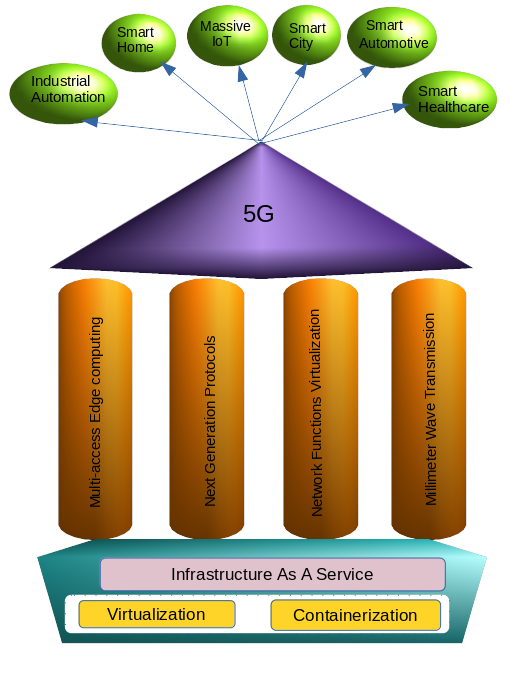
\includegraphics[width=10cm,height=15cm]{5g_pillars}
	\label{fig:figure1}
	\caption{Pillars of 5G Technology}
\end{figure}

\subsection{What is MEC?}

End-user devices have limited resources for computation. Offloading the processing all the way to the cloud introduces problems like network delays, congestion and in degraded quality of service. Hence for applications that need real-time computations, edge computing provides a reasonable solution. The edge nodes are sufficiently powerful and are close to the end-user devices, hence solving both the problems.

MEC (Multi-access Edge Computing) refers to the method of transferring computational complexity which was traditionally handled by server farms and Cloud onto the edge devices that directly interact with the end-user devices. The example of such an application is vehicular traffic management by using real-time data from the sensors consolidated on edge devices at major traffic junctions. A similar example is that of a smart-home environment which has several end-devices controlled by an edge router. 

\subsection{Benefits of MEC}
MEC provides several benefits in realizing traditional and new forms of services to end-user consumers. The major benefits include:

\begin{enumerate}
	\item Computational Offloading
	    \begin{itemize}
		\item Handheld devices with limited processing and data storage capabilities can offload part of the processing to the edge devices without the overhead of transferring the data all the way to the Cloud or Server farms for computational capabilities.
		\item Also, the edge devices that perform the computation have the advantage of access to real-time data from the devices which enables providing new type of services.
		\item Example: Video processing at the edge devices can provide a real-time playback of live events like sports on consumer devices. 
	    \end{itemize}
	\item Service Scalability
	    \begin{itemize}
		\item Due to virtualization and/or containerization of services, its simpler to add new services or extend existing services by adding additional resources.	 
	    \end{itemize}
        \item Service mobility and continuity
    	    \begin{itemize}
                \item Applications involving mobile devices (eg: vehicular devices, smartphones) need persistent service delivery when the devices are in motion. The handover process as the device moves, is simpler when migrating across edge devices.
            \end{itemize}
        \item Service Monetization
    	    \begin{itemize}
                \item Edge computing provides a platform for monetization of the edge infrastructure by allowing third-party applications and services.
            \end{itemize}
\end{enumerate}

With these benefits MEC is set to enable new verticals like video analytics, location services, IoT, Augmented Reality, Real-time Content distribution and data caching for improved web performance. 

\subsection{MCC vs MEC}

MCC or Mobile Cloud Computing can be considered as the technology of the current generation while MEC is an evolution towards the next generation. Several limitations were realized with the current generation MCC in realizing services mainly due to the distance between the user terminal which generates the data and the computational resources that reside in the cloud and use the data to produce useful results. There are also limitations in mobility, scalability and reliability of services which was caused mainly due to communication failures and expensive maintenance cycles. The below table (derived from \cite[p.1628]{mach17}) and the following Kiviat representation provides a comparison of MCC and MEC on key parameters.


\begin{longtable}[H]{|p{0.2\textwidth}|p{0.2\textwidth}|p{0.2\textwidth}|p{0.2\textwidth}|p{0.2\textwidth}|}
\hline\hline
Technical Aspect&MCC&Edge Computing&MCC Weight&MEC Weight\\
\hline\hline
\hline
Deployment&Centralized&Distributed&Not Applicable&NotApplicable\\
\hline
Distance To the UE&High&Low&10.0&2.0\\
\hline
Latency&High&Low&10.0&2.0\\
\hline
Jitter&High&Low&10.0&2.0\\
\hline
Computational Power&Ample&Limited&8.0&4.0\\
\hline
Storage Capacity&ample&Limited&8.0&4.0\\
\hline
\hline\hline

\caption{A Weighted comparison of MCC and MEC\@. Derived from \cite[p.1628]{mach17}}
\label{tab:tab1}
\end{longtable}

\begin{tikzpicture}

\tkzKiviatDiagram[scale=0.5,label distance=3cm,radial=12,gap=1,lattice=12]
	{Distance To UE,Latency,Jitter,Computational Power,Storage Capacity}
\tkzKiviatLine[ultra thick,color=green,mark=ball,mark size=4pt,
               fill=green!20,opacity=.5](10.0,10.0,10.0,8.0,8.0)
\tkzKiviatLine[ultra thick,color=red,mark=ball,mark size=4pt,
               fill=red!20,opacity=.5](2.0,2.0,2.0,4.0,4.0) 
\tkzKiviatGrad[prefix=,unity=1](1)  
\end{tikzpicture}
